% !TEX TS-program = pdflatex
% !TEX encoding = UTF-8 Unicode

\documentclass[a4paper, titlepage=false, parskip=full-, 10pt]{scrartcl}

\usepackage[utf8]{inputenc}
\usepackage[T1]{fontenc}
\usepackage[english, ngerman]{babel}
\usepackage{babelbib}
\usepackage{hyperref}
\usepackage{listings}
\usepackage{framed}
\usepackage{color}
\usepackage{graphicx}
\usepackage[normalem]{ulem}
\usepackage{cancel}
\usepackage{amsmath}
\usepackage{amssymb}
\usepackage{amsthm}
\usepackage{algorithm}
\usepackage{algorithmic}
\usepackage{geometry}
\usepackage{subfigure}
\geometry{a4paper, top=20mm, left=35mm, right=25mm, bottom=40mm}

\newcounter{tasknbr}
\setcounter{tasknbr}{1}
\newenvironment{task}[1]{{\bf Aufgabe \arabic {tasknbr}\stepcounter{tasknbr}} (#1):\begin{enumerate}}{\end{enumerate}}
\newcommand{\subtask}[1]{\item[#1)]}

% Listings -----------------------------------------------------------------------------
\definecolor{red}{rgb}{.8,.1,.2}
\definecolor{blue}{rgb}{.2,.3,.7}
\definecolor{lightyellow}{rgb}{1.,1.,.97}
\definecolor{gray}{rgb}{.7,.7,.7}
\definecolor{darkgreen}{rgb}{0,.5,.1}
\definecolor{darkyellow}{rgb}{1.,.7,.3}
\lstloadlanguages{C++,[Objective]C,Java}
\lstset{
escapeinside={§§}{§§},
basicstyle=\ttfamily\footnotesize\mdseries,
columns=fullflexible,
keywordstyle=\bfseries\color{blue},
commentstyle=\color{darkgreen},      
stringstyle=\color{red},
numbers=left,
numberstyle=\ttfamily\scriptsize\color{gray},
breaklines=true,
showstringspaces=false,
tabsize=4,
captionpos=b,
float=htb,
frame=tb,
frameshape={RYR}{y}{y}{RYR},
rulecolor=\color{black},
xleftmargin=15pt,
xrightmargin=4pt,
aboveskip=\bigskipamount,
belowskip=\bigskipamount,
backgroundcolor=\color{lightyellow},
extendedchars=true,
belowcaptionskip=15pt}

%% Enter current values here: %%
\newcommand{\lecture}{Computer Vision WS15/16}
\newcommand{\tutor}{}
\newcommand{\assignmentnbr}{6}
\newcommand{\students}{Julius Auer}
%%-------------------------------------%%

\begin{document}  
{\small \textsl{\lecture \hfill \tutor}}
\hrule
\begin{center}
\textbf{Übungsblatt \assignmentnbr}\\
[\bigskipamount]
{\small \students}
\end{center}
\hrule

\begin{task}{Lucas-Kanade}
\item[]
\emph{\begin{itemize}
\item Lies das Paper von Lucas und Kanade (1981).
\item Implementiere den Lucas-Kanade-Tracker für rigide Transformationen
\item Tracke die Punktfeatures, die in der Datei ''corners.csv'' gegeben wurden im Video ''beedance.avi'', oder alternativ in einem selbst-gewählten Video.
\item Plotte die Punkttrajektorien auf weißem Hintergrund (Abgabe 1.1)
\end{itemize}}

Dieses Mal implementiere ich den Algo aus Zeitmangel ausnahmsweise nicht selbst und greife stattdessen auf die \emph{OpenCV}-Lösung zurück. Abbildung \ref{fig:1} zeigt die gewünschten Trajektorien, ein lustiges Video (auf jedem Frame sind die Ecken als grüne Punkte markiert) habe ich mit hochgeladen. Ist alles mehr oder weniger default - mir fällt nichts ein, was hier dokumentiert werden müsste.

\begin{figure}[!htpb]
\centering
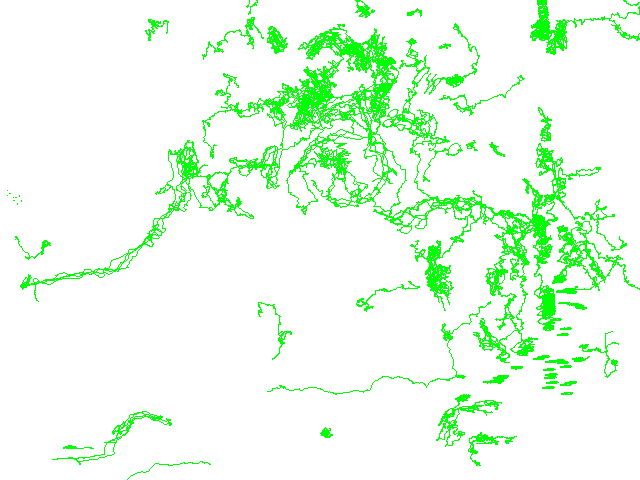
\includegraphics[width=0.9\linewidth]{capture}
\caption{Trajektorien}
\label{fig:1}
\end{figure}
\end{task}
\end{document}